This section will outline the approaches taken to develop and compare a suite of
classifier models as well as the gathering and preparation of a custom coffee
bean defect dataset.

\section{Sample gathering and dataset development}
\label{sec:sample-gathering-and-dataset-development} At the early stages of the
project, it became clear that public coffee bean image datasets will not be suitable
for the aims of this project as they often lack in variety of defects as well as
suffer from a lack of labelling in that regard. Therefore, a custom dataset,
reflecting the variety of existing defects and coffee varieties was necessary to
ensure that any developed model can cope with the diversity of coffee available
on the market.

The gathered dataset consisted of roughly two kilograms of roasted coffee, gathered
from two small-scale coffee roasters: Harmony Roasters based in York and Vibe
With coffee based in Nottingham. Both roasters are in the specialty coffee market
and switch their offerings frequently, allowing them to work with a variety of
coffee suppliers and species. Both roasters mentioned performing manual quality control
after every roast session and expressed interest in the automation of this process,
echoing the research aims of the project.

Over a period of 6 weeks between november and february 2023, both roasters were asked
to keep track of any defective beans they come across and separate the defects by
the variety the coffee belonged to. This ensured that the roasters were not
asked to spend too much of their time and could still perform their usual duties
with as little distraction as possible. Neither roaster asked for compensation for
their work, however, samples of non-defective beans were purchased for their usual
retail price, ensuring that the research process would not take any advantage of
their time and effort.

Upon gathering the beans, the defective beans were inspected once again with each
defect separated into its own section. The separation was done after a
consultation with the coffee roasters, who provided a verbal description of each
defect's visual characteristics. The non-defective beans were also double-checked
for any defects in order to ensure the least amount of incorrectly labelled
samples.

To digitize the dataset, beans of each group were arranged in $5 \times 5$ grids
(where possible) and photographed using the main lens of the Pixel 7 pro smartphone.
Images of each defect were stored locally on the smartphone with a backup made
in google images and GitHub.

Overall, the dataset contained 2786 images, each annotated with the bean variety,
the processing method used and the defect (or lack thereof) present in the bean.
A further description of the dataset is provided below.

\subsection{Dataset description and statistics}
\label{subsec:dataset-description-and-statistics}

\begin{figure}
	{\textwidth}
	\begin{subfigure}
		{0.3\textwidth}
		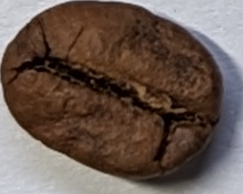
\includegraphics[height=0.8\linewidth, keepaspectratio]{
			./figures/methodology/quaker-bean
		}
		\subcaption{A quaker bean} \label{fig:quakerBeanSingle}
	\end{subfigure}
	\begin{subfigure}
		{0.3\textwidth}
		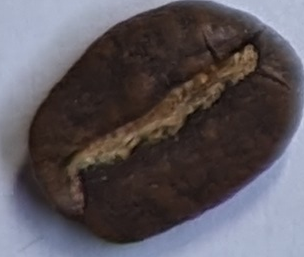
\includegraphics[height=0.8\linewidth, keepaspectratio]{
			./figures/methodology/normal-bean
		}
		\subcaption{A normal bean} \label{fig:normalBeanSingle}
	\end{subfigure}
	\begin{subfigure}
		{0.3\textwidth}
		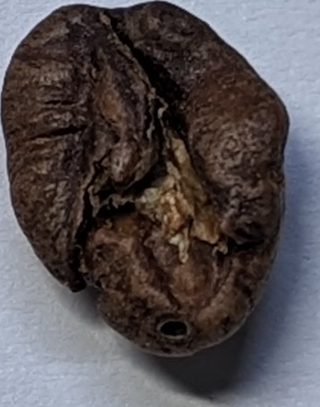
\includegraphics[height=0.8\linewidth, keepaspectratio]{
			./figures/methodology/insect-damaged-bean
		}
		\subcaption{An insect damaged bean} \label{fig:insectBeanSingle}
	\end{subfigure}
	\begin{subfigure}
		{0.3\textwidth}
		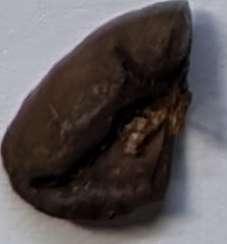
\includegraphics[height=0.8\linewidth, keepaspectratio]{
			./figures/methodology/bean-fragment
		}
		\subcaption{A bean fragment} \label{fig:fragBeanSingle}
	\end{subfigure}
	\begin{subfigure}
		{0.3\textwidth}
		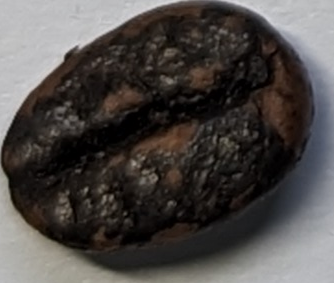
\includegraphics[height=0.8\linewidth, keepaspectratio]{
			./figures/methodology/burnt-bean
		}
		\subcaption{A burnt bean} \label{fig:burntBeanSingle}
	\end{subfigure}
	\begin{subfigure}
		{0.3\textwidth}
		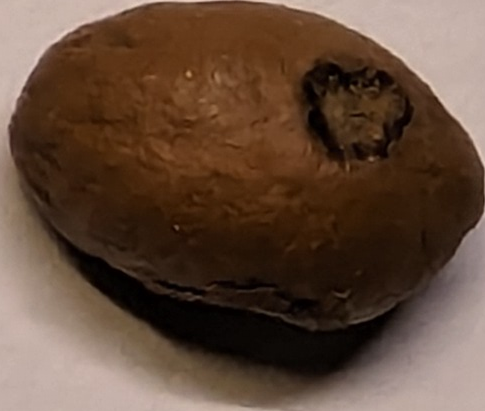
\includegraphics[height=0.8\linewidth, keepaspectratio]{
			./figures/methodology/mold-damaged-bean
		}
		\subcaption{A mould damaged bean} \label{fig:moldBeanSingle}
	\end{subfigure}
	\begin{subfigure}
		{0.3\textwidth}
		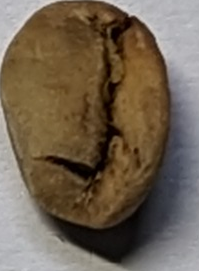
\includegraphics[height=0.8\linewidth, keepaspectratio]{
			./figures/methodology/under-bean
		}
		\subcaption{An underroasted bean} \label{fig:underBeanSingle}
	\end{subfigure}
	\caption{Examples of bean defects}
	\label{fig:beanDefects}
\end{figure}

\subsection{Approach to data gathering and pre-processing}
\label{subsec:approach-to-data-gathering-and-pre-processing}

\section{Combatting class imbalance}
\label{sec:combatting-class-imbalance}

\section{Approaches to model development}
\label{sec:approaches-to-model-development}
\subsection{Dimensionality reduction techniques for KNN classification}
\label{subsec:dimensionality-reduction-techniques-for-knn-classification}

\section{Model development results}
\label{sec:model-development-results}